\documentclass[conference]{IEEEtran}
\usepackage{cite}
\usepackage{amsmath,amssymb,amsfonts}
\usepackage{algorithmic}
\usepackage{booktabs}
\usepackage{graphicx}
\usepackage{textcomp}
\usepackage{xcolor}
\usepackage[colorlinks,linkcolor=blue]{hyperref}
\def\BibTeX{{\rm B\kern-.05em{\sc i\kern-.025em b}\kern-.08em
		T\kern-.1667em\lower.7ex\hbox{E}\kern-.125emX}}
\begin{document}
	
	\title{AI3607: Deep Learning Course Assignment \\ JPG: Solving Jigsaw of all Permutations with GAN  \\
		{\normalsize \vspace{1em} Kailing Wang(\href{mailto:wangkailing151@gmail.com}{Email}) \\ Shanghai Jiao Tong University \\ 2023.5.15}
	}
	
	\maketitle
	
	\begin{abstract}
		In this report, I proposed a framework for solving jigsaw puzzles. Unlike some naive methods using only simple networks, my method is composed of more functional blocks, and additionally, my method supports unsupervised learning and has the potential for solving puzzles with more pieces. Moreover, my framework is specially designed for datasets of low resolution like CIFAR10 but should perform even better on large datasets.
	\end{abstract}
	
	\begin{IEEEkeywords}
		Jigsaw, GAN, Flow-map, Unsupervised Learning
	\end{IEEEkeywords}
	
	\section{\textbf{Introduction}}
	There aren't many solving jigsaw puzzles successfully before as a recent paper review\cite{0}. Santa at el. performed a multi-functional network\cite{1}, but can only solve jigsaws with few pieces. Paumard et al. used local features and achieved a good result\cite{2}, but they need pictures of higher resolution. The work of R. Le et al. showed a method using a complete GAN to solve jigsaw puzzles\cite{3}. They generate pictures from shuffled pieces and evaluate how much it is possibly wrongly arranged, but they train on limited permutations of a puzzle. Here I propose a simpler version of JigsawGan but use all possible permutations of a puzzle, which is considered hard to achieve good results. 
	
	\section{Task Analysis}
	The task of our course assignment is to do puzzle-solving on CIFAR10. 
	\subsection{Potential Solutions}
	Before I build up my method, I considered several alternatives and modifications:
	\subsubsection{Naive Method}The recommended methods only use some simple convolution layers and some linear layers to train a one-hot position code for an Input image. Some tried to use ResNet to replace the convolution network and claim to reach more than 95\% percent accuracy while using only the 64-dimensional output from ResNet as features, which I consider impossible: that loses too much information.
	
	\subsubsection{Resize}
	Some others resize the datasets larger as a whole, which significantly improved the performance. However, this is a fatal mistake. If you resize the whole image, you are adding prior information to the test datasets. Let's consider a naive jigsaw solver for jigsaws of 4 pieces: since jigsaw pieces are cut from a continuous image, the pixels should be almost continuous on the edges across each block piece. That is, we can solve the puzzle by solving the optimization problem below:
	\begin{equation}
		\min_{i\in \{\mathcal P\}} \operatorname{T V}(\text{img}[i])
	\end{equation}
	where $i$ is a arrangement sequence from all possible permutations $\mathcal P$ and img[$index$] is rearranged image. $\operatorname{TV}$ is the total variation. In fact, we only compute total variation on the edges(see fig. \ref{p1}.). I implemented this method on CIFAR10 and the results are in table \ref{t1}. As we can see, directly resizing 32 to 64 makes accuracy significantly higher, and even more if to 128. If we resize each block from 16 to 32, the change in accuracy is minor. I claim the result of those trying to resize the whole image is invalid. The showed result also provides a baseline, that we should reach about 80.33\% using naive networks.
	
	\begin{figure}[h!]
		\centering
		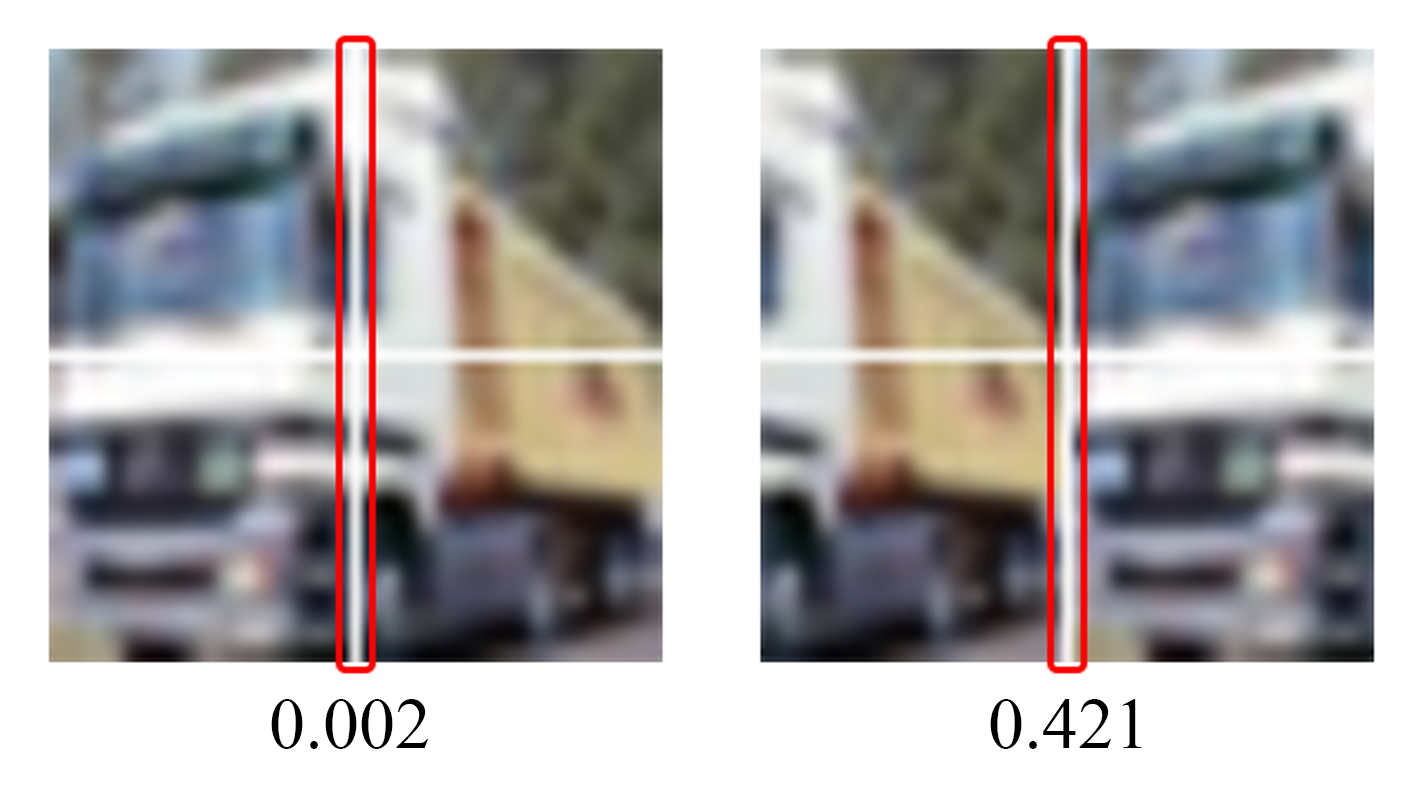
\includegraphics[width=0.8\linewidth]{figures/edgeloss}
		\caption{Total Variation Compare}
		\label{p1}
	\end{figure}
	
	\begin{table}[htbp]
		\caption{Optimization Method Accuracy}
		\centering
		\begin{tabular}{cc}
			\toprule
			Resolution Method & Accuracy on full CIFAR10 \\
			\midrule
			original image & 80.33\% \\
			whole image 32 to 64 & 91.67\% \\
			image piece 16 to 32 & 81.79\% \\
			whole image 32 to 128 & 95.88\% \\
			\bottomrule
		\end{tabular}
		\label{t1}
	\end{table}
	
	\subsubsection{Edge Weight}
	As I have shown, edge loss is rather important, so consider adding weight on piece edges should be useful. However, the content inside the image also counts so the weight should be minor. I propose a loss to replace this edge effect. 
	
	\begin{figure*}[t]
		\centering
		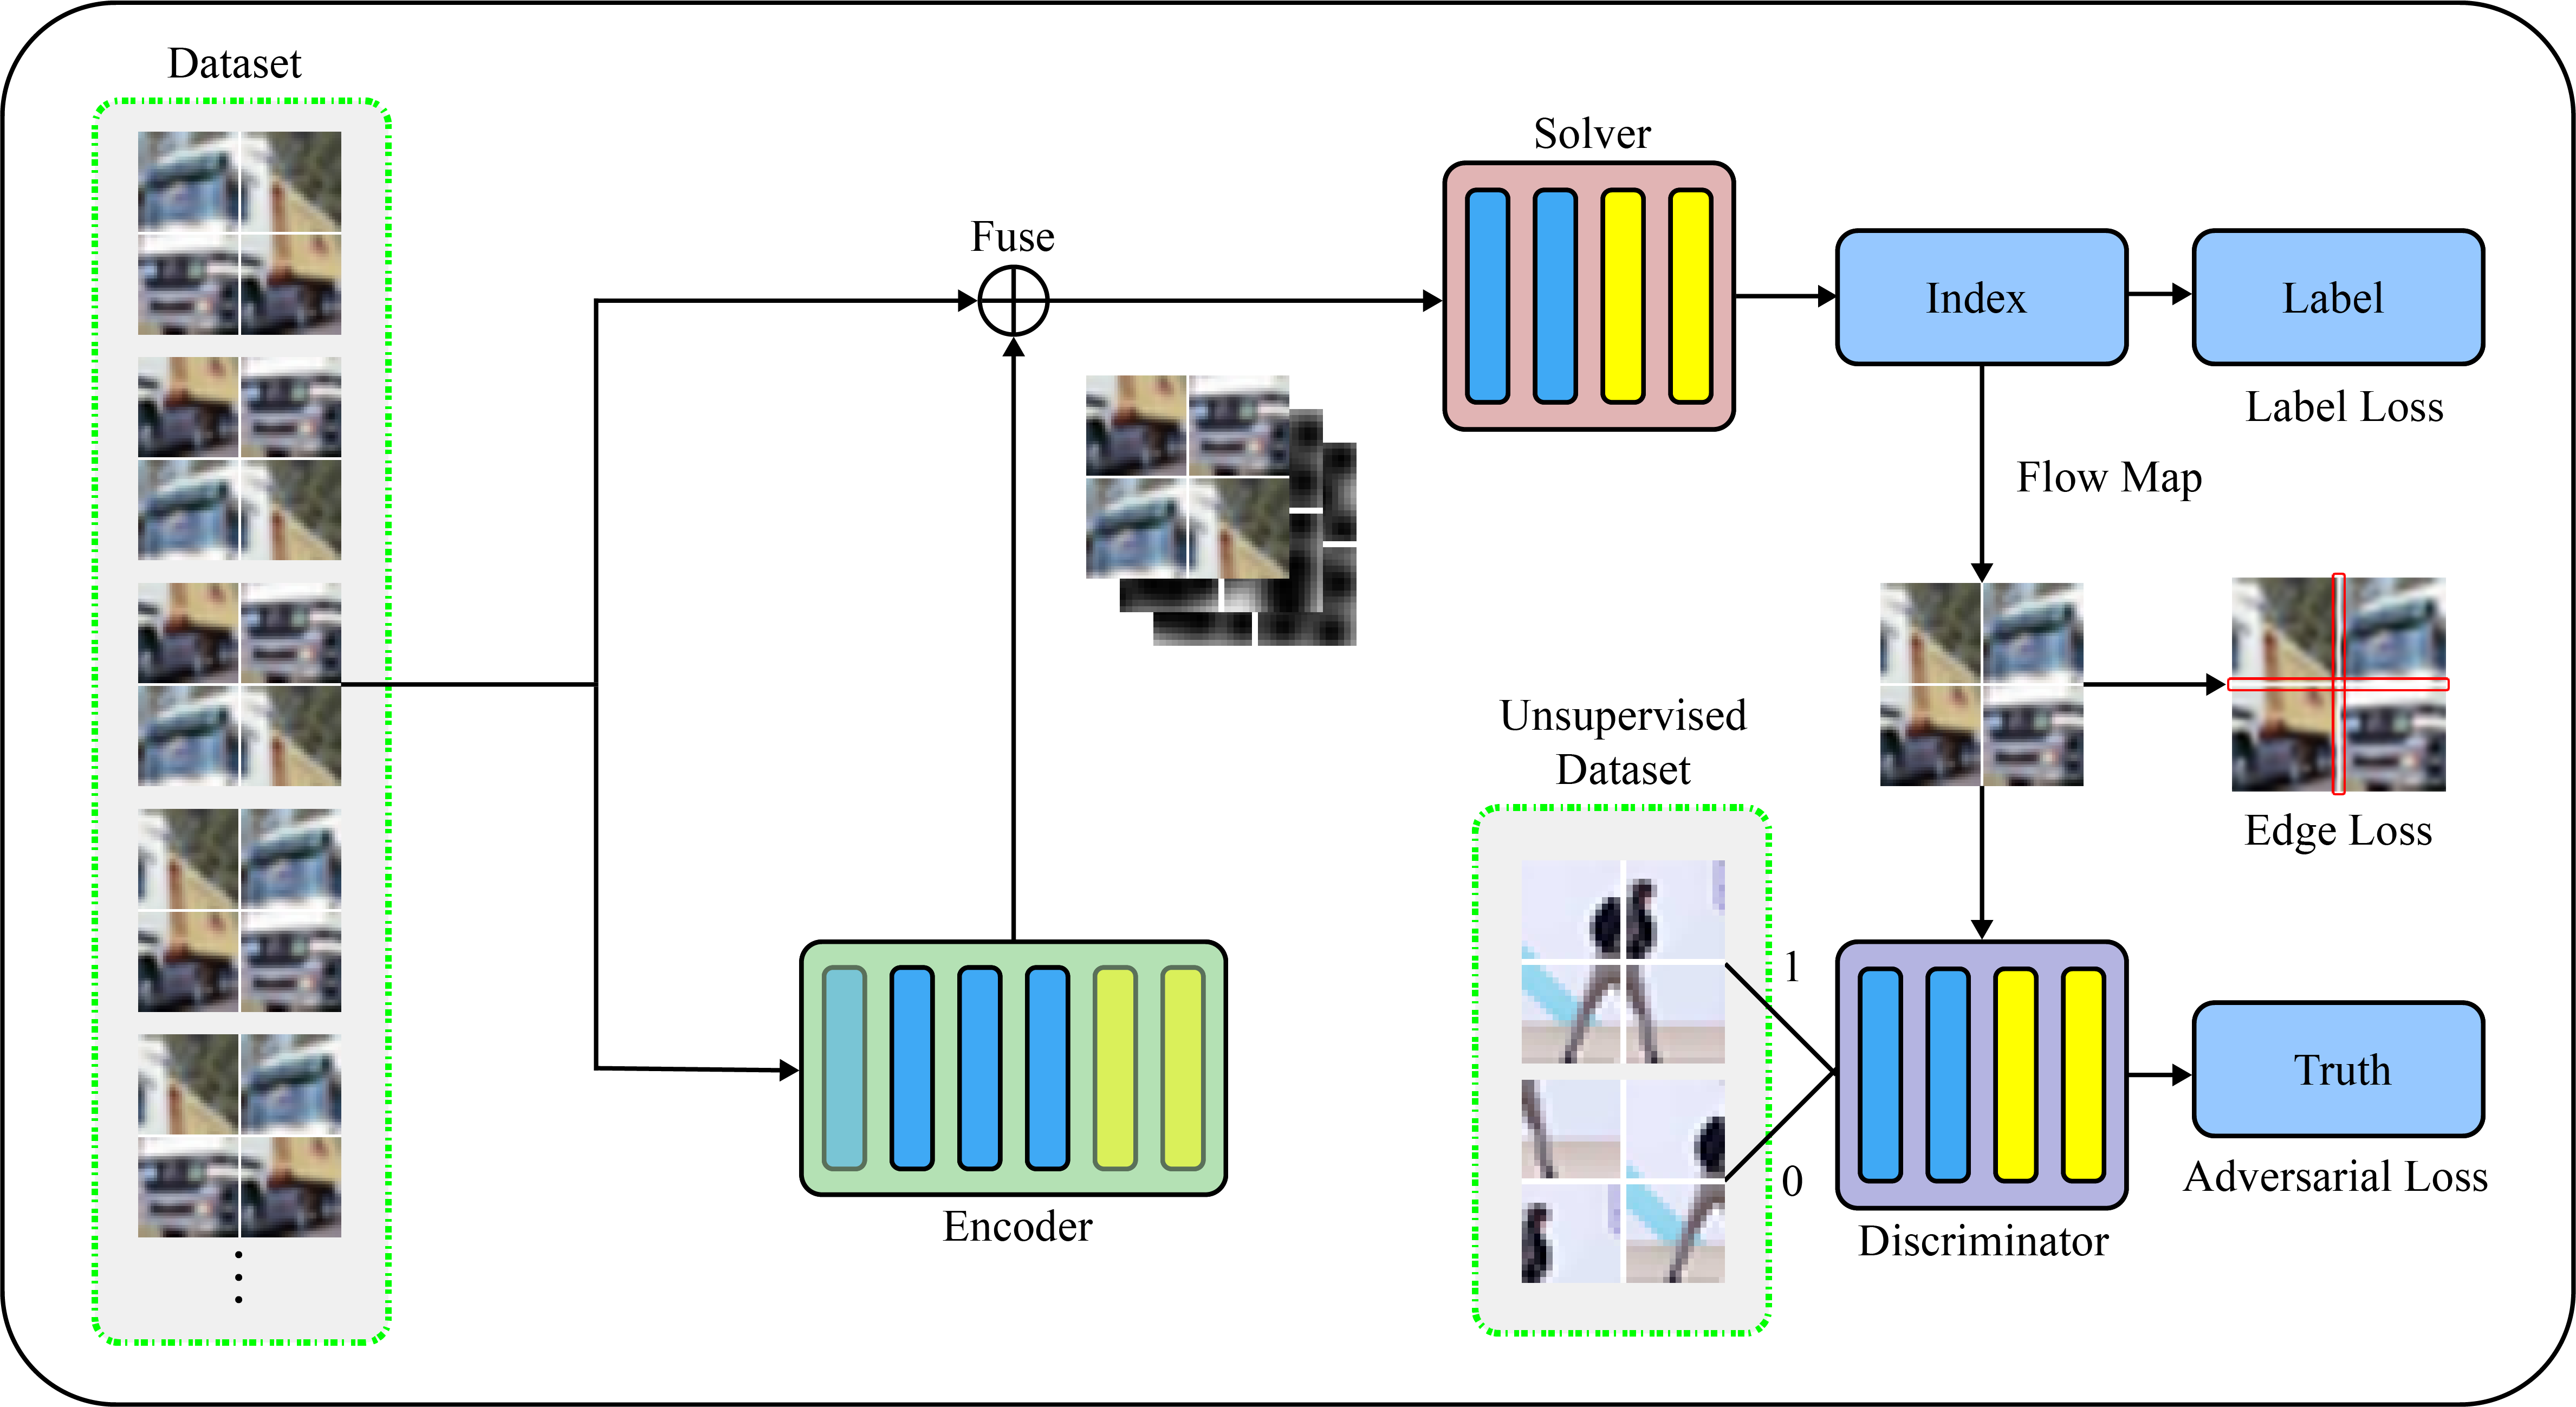
\includegraphics[width=\textwidth]{figures/pipline}
		\caption{The datasets include different jigsaws generated from a single figure. The encoder is the convolution layer of a CIFAR10 classifier if pre-trained. The output fused with the raw input is fed into the solver. The discriminator is a classifier that classifies if an image is correctly arranged.}
		\label{pip}
	\end{figure*}
	
	\subsection{Data}
	There are a few points to explain before we give a further solution.
	\subsubsection{Jigsaw generation}
	CIFAR10 includes 50000 train images and 10000 test images. When we cut the image into 4 pieces, there are 24 permutations for each image and the dataset is now with 1.2 million of training data and 240 thousand of test data. However, when we cut the image to 9 pieces or more, the size is not affordable, i.e. $9! = 362,880$.
	\subsubsection{Resolution}
	As I mentioned before, 
	\section{\textbf{Methods}}
	The pipeline of my method is shown as fig \ref{pip}. When the image is cut into 4 pieces, the datasets include all 24 permutations of each image. The data is first encoded by an encoder. The encoder can be either randomly initialized or pre-trained as a classifier, but will not be trainable during the main process. Details will be explained in part  \uppercase\expandafter{\romannumeral4}. The encoded features are fused with the input data and then feed into the solver which then generates a sequence. The discriminator is trained not necessarily trained on given datasets but can be trained unsupervised on any data. The design of the discriminator is inspired by the real GAN model. In fact, when training unsupervised, the discriminator can be trained further in the main process and function just like that in GAN.
	\subsection{Network Architecture}
	Considering we are designing a method for images with lower resolution, the network shouldn't be large. The blue layers in fig \ref{pip} refer to convolution and yellow linear. As we can see, the decoder is three convolutions with 32, 32, and 64 filters each. The discriminator is composed of two convolution layers with 8 and 16 filters, and two linear layers with 4096 hidden. The solver's convolution layers have 64, 64 filters each, and linear layers also 4096. All the mentioned filters are set to size 3, 1 padding, and 1 stride. 
	\subsection{Flow Map Transition}
	The output from the solver is a list of index sequences. In order to fetch some information inside the image, there should be a way to pass the gradient into the image. If I'm using torch, I can just convert the sequence to int type and calculate the movement of each piece to form a flow map that has the desired gradient. Then we multiply the flow map with the input image to get the output image. However, jittor will desert the gradient in such a process. The alternative solution is to directly multiply the normalized index sequence to the image pieces like fig \ref{p2}.
	\begin{figure}[h!]
		\centering
		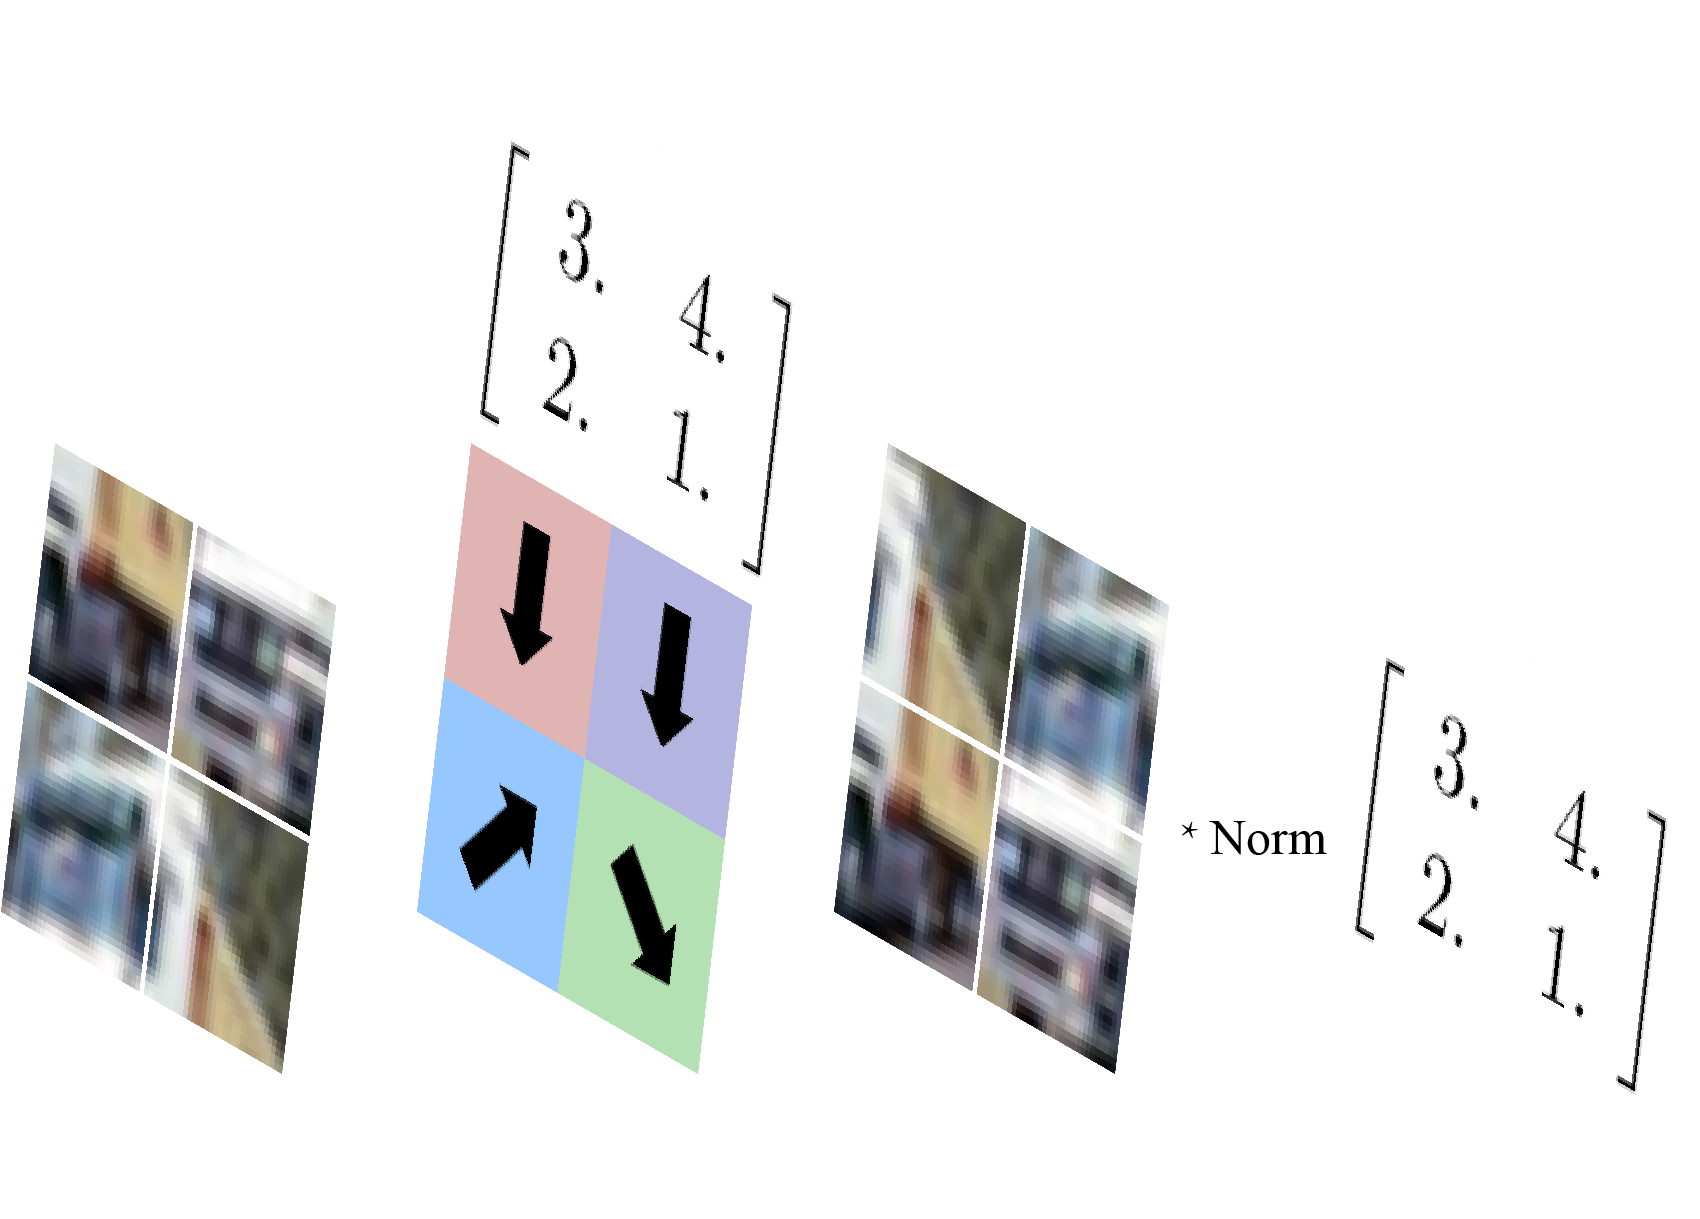
\includegraphics[width=0.8\linewidth]{figures/flow}
		\caption{Total Variation Compare}
		\label{p2}
	\end{figure}
	\subsection{Loss Function}
	\subsubsection{Label Loss}
	When we are training on CIFAR10, we have the original image and we generate the correct label while training. The obvious loss function is:
	\begin{equation}
		\mathcal L_l (X, label) = ||\operatorname{Model}(X) - label||_1
	\end{equation}
	Where X is the data, the model is the inference part of my framework and the label is the target.
	\subsubsection{Edge Loss}
	Edge information counts. In the last subsection, I show my way to pass the gradient into the output image, so we can calculate the total variation of the image as loss:
	\begin{equation}
		\mathcal L_e (X) = \operatorname{TV}(\operatorname{Image}(X, \operatorname{Model}(X)))
	\end{equation} 
	Where the Image is to rebuild the image with the output. 
	\subsubsection{Discriminator Loss}
	The discriminator decides if the out image is a real image. I imitate GAN to pass loss:
	\begin{equation}
		\mathcal L_d (X) = \operatorname{Image}(X, \operatorname{Model}(X)) * \operatorname{D}(\operatorname{Image}(X, \operatorname{Model}(X)))
	\end{equation}
	Where $D$ is the discriminator. 
	
	The total loss is:
	\begin{equation}
		\mathcal L = \alpha\cdot L_l+\beta\cdot L_e+\gamma\cdot L_d
	\end{equation}
	\subsection{Additional or Potential}
	\subsubsection{Unsupervised}
	The discriminator does not depend on the jigsaw datasets. It can be trained on any real-world image set. When we come across jigsaw puzzles that do not have the original image, let's say, solving real puzzles the answer maps are lost (dismiss the difference of non-edge jigsaws). 
	\subsubsection{Extremely Low Resolution}
	CIFAR10 itself is a case. When cut into 16, each piece is $8\times 8$, and feature extraction is rather hard. The discriminator loss helps to seek more semantic information and goes beyond labels.
	\subsubsection{Bad Label Mislead}
	If the datasets can't ensure all the labels are correct, labels could mislead the solver. In other cases, if a large image contains the image of a sky, white walls, or sea, there could be interchangeable pieces. An extreme example is a picture containing a mass area of pure white. The discriminator will avoid learning if the outcome is considered valid. 
	\section{\textbf{Implementation Details}}
	I've tried to implement the code as elegant and standard as I could as a complete project. Aside from traditional implementation detail explanation, I will also add what should be in README.md. 
	\subsection{Training Process}
	There is an option whether to use the encoder or not, for the convolution layers in the solver can also get some features when the data size is small enough. If you choose to use an encoder, there is a problem to consider: should we pre-train the encoder? My answer is we mustn't pre-train because if we pre-train the encoder as a classifier, it is likely to extract similar features from different permutations of the same image, which actually reduces significant features. 
	
	My code supports resizing, and there are two modes of resizing: resizing the whole image(which is actually illegal for the task) and resizing pieces. The discriminator is also optional. The weight of label loss is the majority, and the learning rate declines as label loss gets smaller. The latter two losses will function during the latter half of the training. 
	\subsection{Test Process}
	There are two accuracy methods with respect to solving jigsaws: All in position or One by one. The former means accuracy gains only when the whole image is correctly rebuilt, and the latter means accuracy is viewed for each piece. In my implementation, these two methods have minor differences, but I retain them one by one in the final code only. 
	\subsection{Devices}
	My code detects if you have Cuda devices but could use at most one. Depending on your config, the training time should be around 0.5 to 2 hours on a single RTX4090 but observed faster on a single RTX3080 or even RTX2080Ti. Some significant calculation processes are done on the CPU so the training time will be significantly slower if your batch size is too small or your CPU is busy. If you don't upsize the image too large, the training should only cost 1 to 4 Gib of memory. 
	\section{\textbf{Experiments}}	\begin{table*}[!h]
		\centering
		\caption{Experiments of JPG}
		\begin{tabular}{cccccc}
			\toprule
			Resize & Edge Loss & Discriminator Loss & Encoder & Pretrain & Performance\\
			\midrule
			- & - & - & - & - & 81.70\%\\
			whole image to 64 & - & - & On & - & *93.72\%(Invalid)\\
			pieces to 32& - & - & - & - & 80.60\%\\
			- & - & - & On & - & 82.88\%\\
			- & - & - & On & Yes & 80.62\%\\
			- & 0.01 & - & On & - & 83.18\%\\
			- & - & 0.1 & On & - & 83.03\%\\
			- & 0.01 & 0.1 & On & - & *\textbf{86.49\%}(Advanced)\\
			\bottomrule
		\end{tabular}
		
		* This experiment is done in $draft.ipynb$. In the submitted code,\\the whole image upsize is not allowed, but the argument remains in the concerned functions.\\ *The advanced results are done under a better config
	\end{table*}
	\begin{figure*}[!h]
		\centering
		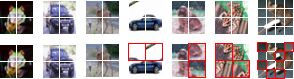
\includegraphics[width=0.8\linewidth]{figures/res}
		\caption{Results}
		\label{p3}
	\end{figure*}
	\subsection{Code Structure}
	As a complete project, I prepared the setup scripts for both Windows and Ubuntu(Linux). There are $init.bat$ and $init.sh$ to automatically create a conda environment and install packages in $requirements.txt$. The code supports passing in config JSON files. I have prepared some configs used in experiments. All the learning options, loss options, and even validate-only are supported arguments. Since I can hardly trust Jittor in some important functions, I implement many tool functions in the $utils.py$. The image cut and shuffle are based on pillow since Jittor uses it, and the JigsawPuzzle dataset is also specially designed for my method. Error info will be logged in the directory with the name of the experiment and models can be saved automatically. The random seed is kept during the experiments, and my model is robust to changes in parameters: it always converges at least. I also tried to implement an animation module in the command line.
	My code actually supports cuts of any piece, but to make it easy to compare, I only showed the results of 4 pieces. Note that my datasets include \textbf{1,200,000} training data and \textbf{240,000} test data. Random seeds are all fixed.

	
	Note that I can't afford to implement other methods, and as I have shown, the performance rises on datasets of higher resolution There isn't a valid baseline on CIFAR10. 
	
	Some of the predicted results are in fig \ref{p3}. I still want to say, that even for humans it is hard to solve jigsaw puzzles with such resolution. Check the 16 pieces case, I can hardly recognize what is it. For 4 pieces cases, errors are more likely to occur when the colors are almost the same across pieces. The image of a car in fig \ref{p3} is an explicit example, in which the two white blocks are incorrectly placed. But in fact, these two pieces contain only minor information and we should allow such mistakes. 
	
	\section{\textbf{Further Works}}
	The GAN part in my method does not include a full GAN. However, in my mind there is a better way to use GAN to further help train: We can actually generate a picture from the result arrangement, and we could use some image compare methods to calculate a real image loss. Some diffusion models may also be helpful.
	\section*{Additional}
	This report was polished by Grammarly but ChatGPT. Inform me if it could not pass the AI detection like GPT-Zero. Also note that some used ChatGPT completely to reach 95\%, which is really confusing. 
	\begin{thebibliography}{99}
		\bibitem{0} Jigsaw puzzle solving techniques and applications: a surve
		\bibitem{1} Santa Cruz R, Fernando B, Cherian A, et al. Deeppermnet: Visual permutation learning[C]//Proceedings of the IEEE Conference on Computer Vision and Pattern Recognition. 2017: 3949-3957.
		\bibitem{2} Paumard M M, Picard D, Tabia H. Jigsaw puzzle solving using local feature co-occurrences in deep neural networks[C]//2018 25th IEEE International Conference on Image Processing (ICIP). IEEE, 2018: 1018-1022.
		\bibitem{3} Li R, Liu S, Wang G, et al. Jigsawgan: Auxiliary learning for solving jigsaw puzzles with generative adversarial networks[J]. IEEE Transactions on Image Processing, 2021, 31: 513-524.
	\end{thebibliography}
\end{document}
